\section{Auswertung}
\subsection{Untersuchung des Linearverstärkers}
In diesem Teil der Auswertung soll das Verhalten der Verstärkung eines invertierenden Linearverstärkers untersucht werden.
Hierzu werden vier Aufbauten mit unterschiedlichen Widerstandskombinationen vermessen.
Der Aufbau erfolgt nach Abbildung \ref{invert} mit den folgenden Widerstandspaaren aus Tabelle \ref{Tab_2}.
Der Verstärkungsfaktor $V_\text{ideal}$ rein aus dem Widerstandsverhältnis für einen idealen Operationsverstärker wird zum Vergleich der erhaltenen Messdaten nach \eqref{eq:V_linear} berechnet; das negative Vorzeichen ergibt sich aus dem invertierenden Verhalten des Verstärkers.
\begin{table}[]
\centering
\begin{tabular}{c|ccc}
&$R_1\,[\si{\kilo\ohm}]$&$R_N\,[\si{\kilo\ohm}]$&Verstärkungsfaktor $V_\text{ideal}$\\
\hline
Verstärker 1 & 100 & 10  &$-1/10$\\
Verstärker 2 & 100 & 1   &$-1/100$\\
Verstärker 3 & 10  & 0,5 &$-1/20$\\
Verstärker 4 & 10  & 33  &$-3{,}3$
\end{tabular}
\caption{Widerstandsparameter der äußeren Beschaltung $R_1$ und $R_2$ der Grundschaltung des invertierenden Verstärkers mit der daraus berechneten Verstärkung $V_\text{ideal}$.}
\label{Tab_2}
\end{table}
Gemessen wurde die Ausgangsspannung $U_A$ in Abhängigkeit der Frequenz $\nu$.
Ermittelt werden soll die Grenzfrequenz $\nu_\text{Grenz}$, bei der die Verstärkung auf einen Faktor $\frac{1}{\sqrt{2}}$ abgefallen ist. Die Verläufe der Verstärkung für die vier Widerstandspaare sind in den Abbildungen \ref{linear1}, \ref{linear2}, \ref{linear3} und \ref{linear4} zusehen.

Für die Verstärker 1, 2 und 3 ist der Absolutbetrag des Logarithmus des Spannungsverhältnis $\frac{U_A}{U_1}$ verwendet worden, da hier eine Verstärkung $|V'|<1$ vorliegt, sodass der direkte Vergleich mit dem Graphen des Verstärkers 4 nicht ohne Weiteres möglich ist. Des Weiteren ist darüber möglich, die Grenzfrequenz $\nu_\text{Grenz}$ direkt zu berechnen, ohne den Definitionsbereich des Logarithmus zu überschreiten.
Die Annahme, dass die Verstärkung direkt proportional zum Verhältnis der Widerstände der äußeren Beschaltung ist, rührt aus der Betrachtung des Operationsverstärkers als ideales Bauteil, sodass sich die Verstärkung nach \eqref{eq:V_linear} ergibt.\\
Für alle vier Beschaltungen wird eine Eingangsspannung von $U_1=\SI{3}{V}$ verwendet.
Zur Bestimmung der Grenzfrequenz $\nu_\text{Grenz}$ und des Verstärkung-Bandbreite-Produkts $V_0\nu_\text{Grenz}$ wird zunächst der konstante Verlauf der experimentellen Kennlinie untersucht. Aufgrund des anzunehmenden konstanten Wertes, wird jeweils der Mittelwert der in den Graphen als orange eingezeichneten Messwerte $\bar{V}_0$ gebildet.
Für die Bestimmung der Grenzfrequenz $\nu_\text{Grenz}$ wird eine lineare Ausgleichsrechnung der Form
\begin{equation}
  f(x)=mx^b
\end{equation}
erstellt, um die Steigung des doppellogarithmischen Plots zu bestimmen.
Hierüber lässt sich mittels
\begin{equation}
  \nu_\text{Grenz}=\exp(\ln(V_0/\sqrt{2})-b/m)
\end{equation}
die Grenzfrequenz bestimmen sowie schließlich das Verstärkung-Bandbreite-Produkt $V'\nu_\text{Grenz}$, welches im Idealfall konstant sein soll. Die erhaltenen Ausgleichwerte sowie die daraus bestimmten Kenngrößen sind in Tabelle \ref{Werte_fit} zu finden. Aufgrund des Verlaufs des Graphen in Abbildung \ref{linear1}, für den der Verstärkungsteil auch nach Betragsbildung nicht eindeutig zugeordnet werden kann, bleibt dieser als weiterer Vergleichswert fragwürdig.

\begin{table}[H]
  \small
\centering
\begin{tabular}{c|ccccc}
&$m\,[\frac{1}{\si{\ln(\mathrm{Hz)}}}]$ & $b$ & $\ln(\bar{V}_0)$ & $\nu_\text{Grenz}\,[\mathrm{Hz}]$ & GBP$\,[\mathrm{Hz}]\, (V_0\nu_\text{Grenz})$\\
\hline
Verstärker 1 & $\si{0,776\pm0,008}$ & $-\si{7,97\pm0,10}$ & $\si{2,275}$ & $(5{,}3 \pm 0{,}9) \cdot 10^{4}$ & $(1{,}21 \pm 0{,}21) \cdot 10^{5}$\\
Verstärker 2 & $-\si{0,756\pm0,028}$ & $\si{14,1\pm0,4}$ & $\si{4,423}$ & $(2{,}8 \pm 2{,}3) \cdot 10^{7}$ & $(1{,}2 \pm 1{,}0) \cdot 10^{8}$\\
Verstärker 3 & $-\si{0,248\pm0,009}$ & $\si{4,69\pm0,07}$ & $\si{2,989}$ & $(8{,}0 \pm 6{,}0) \cdot 10^{6}$ & $(2{,}5 \pm 1{,}6) \cdot 10^{7}$\\
Verstärker 4 & $-\si{0,815\pm0,010}$ & $\si{8,86\pm0,11}$ & $\si{0,143}$ & $(8{,}8 \pm 1{,}9) \cdot 10^{5}$ & $(1{,}25 \pm 0{,}27) \cdot 10^{5}$\\
\end{tabular}
\caption{Ergebnisse der linearen Ausgleichsrechnung und der mittels dieser berechneten Werte der Grenzfrequenz $\nu_\text{Grenz}$ und des Verstärkung-Bandbreite-Produkts GBP.}
\label{Werte_fit}
\end{table}

\begin{figure}[h]
  \centering
  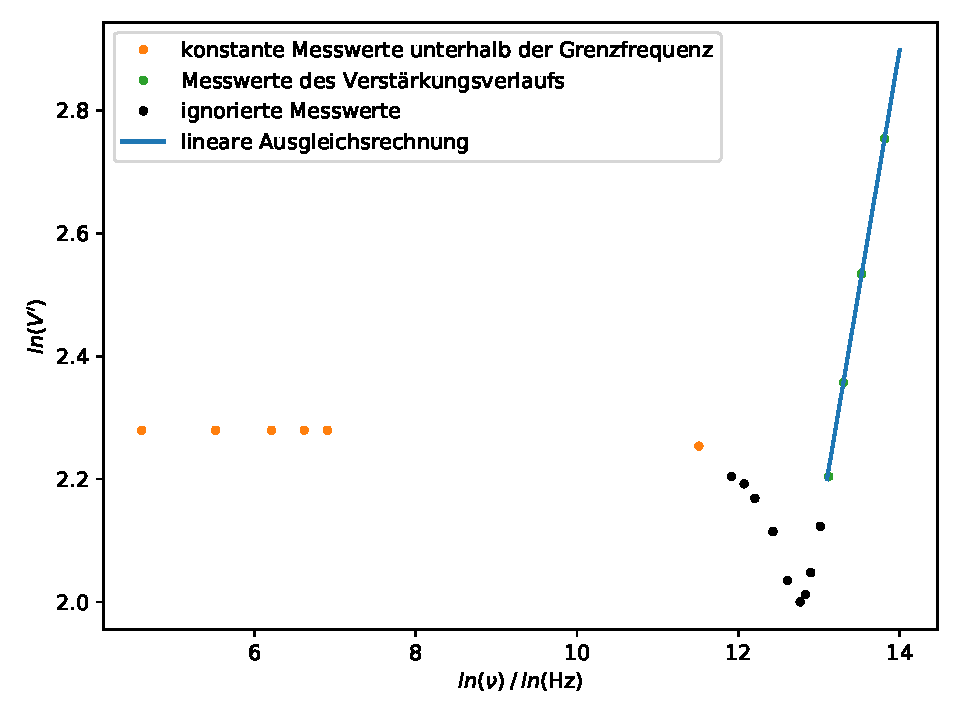
\includegraphics[width=0.62\textwidth]{Linearverstaerker_Anneke/A1.pdf}
  \caption{Graphischer Verlauf des Verstärkungsfaktors $V'$ in Abhängigkeit der Frequenz $\nu$ in doppellograrithmischer Darstellung für den ersten beschalteten Linearverstärker. Die als konstant anzunehmenden Messwerte sind orangefarben markiert worden; die des Verstärkungsverlaufs grün. Für die Auswertung ignorierte Messwerte sind schwarz gezeichnet. Die in blau gezeichnete lineare Ausgleichsrechnung soll die Verstärkung annähern.}
  \label{linear1}
\end{figure}
\begin{figure}[h]
  \centering
  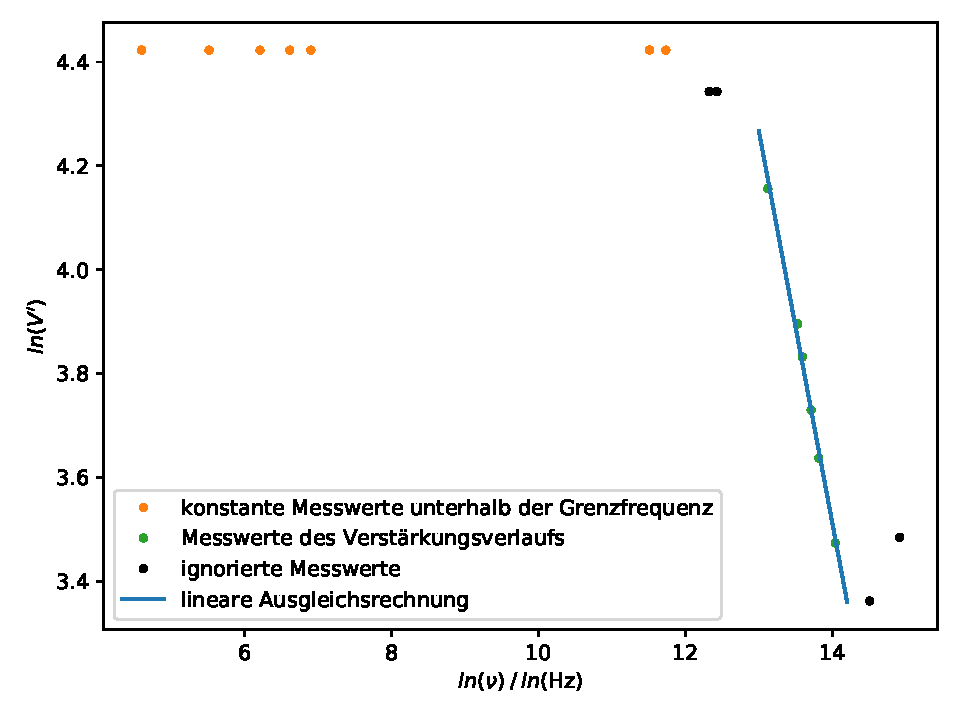
\includegraphics[width=0.62\textwidth]{Linearverstaerker_Anneke/A2.pdf}
  \caption{Graphischer Verlauf des Verstärkungsfaktors $V'$ in Abhängigkeit der Frequenz $\nu$ in doppellograrithmischer Darstellung für den zweiten beschalteten Linearverstärker. Die als konstant anzunehmenden Messwerte sind orangefarben markiert worden; die des Verstärkungsverlaufs grün. Für die Auswertung ignorierte Messwerte sind schwarz gezeichnet.  Die in blau gezeichnete lineare Ausgleichsrechnung soll die Verstärkung annähern.}
  \label{linear2}
\end{figure}
\begin{figure}[h]
  \centering
  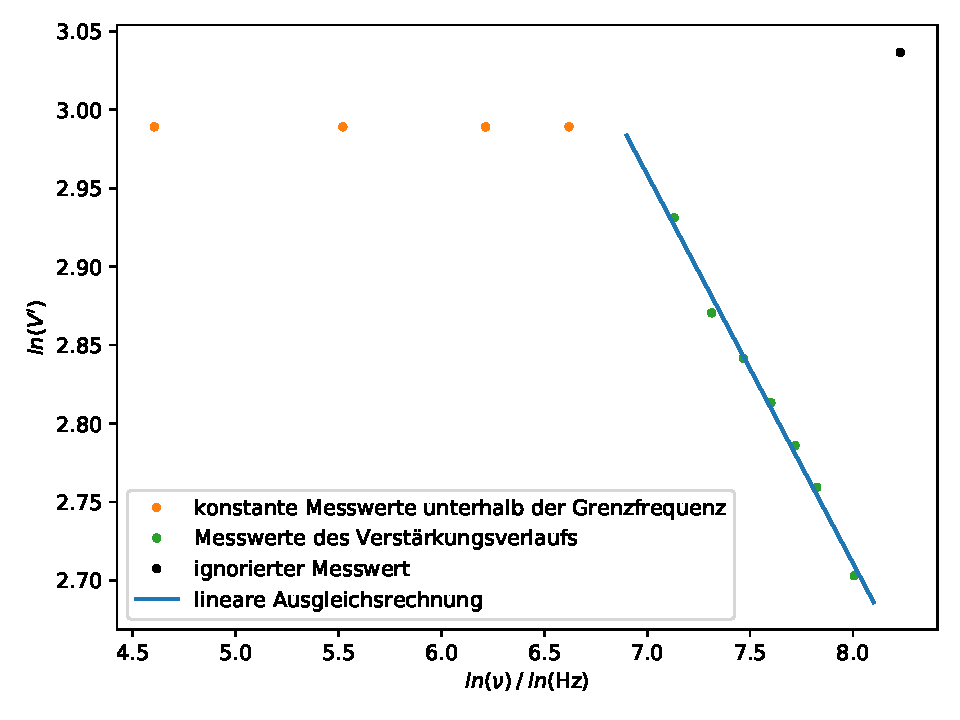
\includegraphics[width=0.65\textwidth]{Linearverstaerker_Anneke/A3.pdf}
  \caption{Graphischer Verlauf des Verstärkungsfaktors $V'$ in Abhängigkeit der Frequenz $\nu$ in doppellograrithmischer Darstellung für den dritten beschalteten Linearverstärker. Die als konstant anzunehmenden Messwerte sind orangefarben markiert worden; die des Verstärkungsverlaufs grün. Für die Auswertung ignorierte Messwerte sind schwarz gezeichnet.  Die in blau gezeichnete lineare Ausgleichsrechnung soll die Verstärkung annähern.}
  \label{linear3}
\end{figure}
\begin{figure}[h]
  \centering
  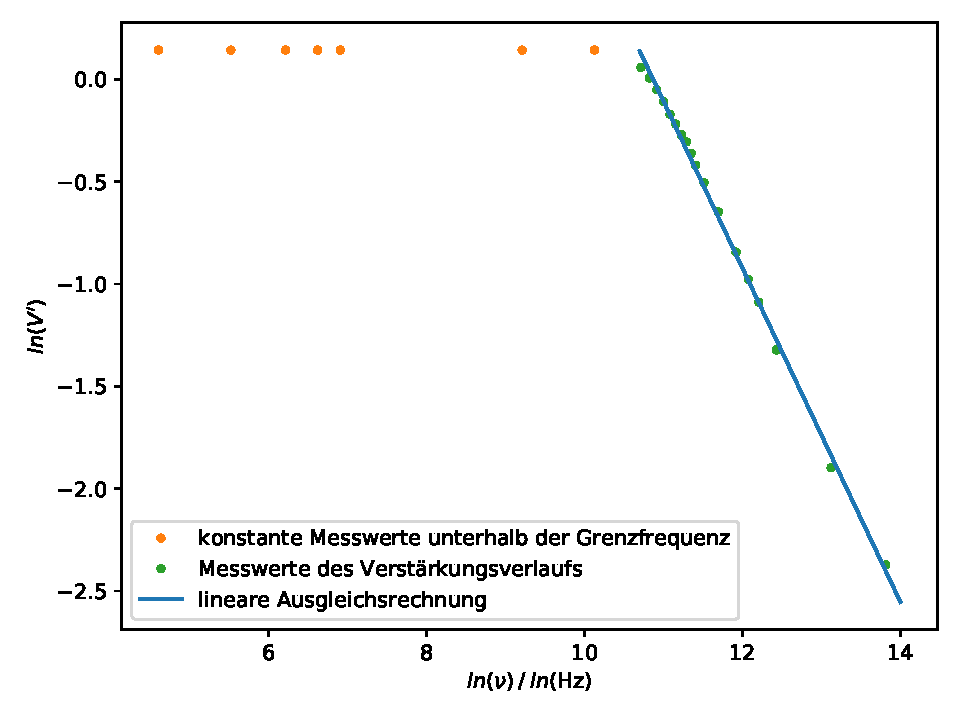
\includegraphics[width=0.65\textwidth]{Linearverstaerker_Anneke/A4.pdf}
  \caption{Graphischer Verlauf des Verstärkungsfaktors $V'$ in Abhängigkeit der Frequenz $\nu$ in doppellograrithmischer Darstellung für den vierten beschalteten Linearverstärker. Die als konstant anzunehmenden Messwerte sind orangefarben markiert worden; die des Verstärkungsverlaufs grün.  Die in blau gezeichnete lineare Ausgleichsrechnung soll die Verstärkung annähern.}
  \label{linear4}
\end{figure}
\clearpage
Für den nächsten Schritt wird die gemessene Phase zwischen der Eingangs- und der Ausgangsspannung $\varphi$ gegen die eingestellte Frequenz $\nu$ aufgetragen. Hierdurch soll die Phasenverschiebung zwischen den beiden Signalen bei ändernder Frequenz untersucht werden. Zu sehen ist dieser Verlauf in Abbildung \ref{phase}.
Erkennbar ist, dass die beiden Signale bei niedrigen Frequenzen einer Phasenverschiebung um $\SI{180}{^\circ}$ unterliegen; Mit steigender Frequenz wird diese abgebaut.
Durch Augenmaß kann hier eine kritische Frequenz von $\SI{10}{kHz}$ bestimmt werden.
\begin{figure}[h]
  \centering
  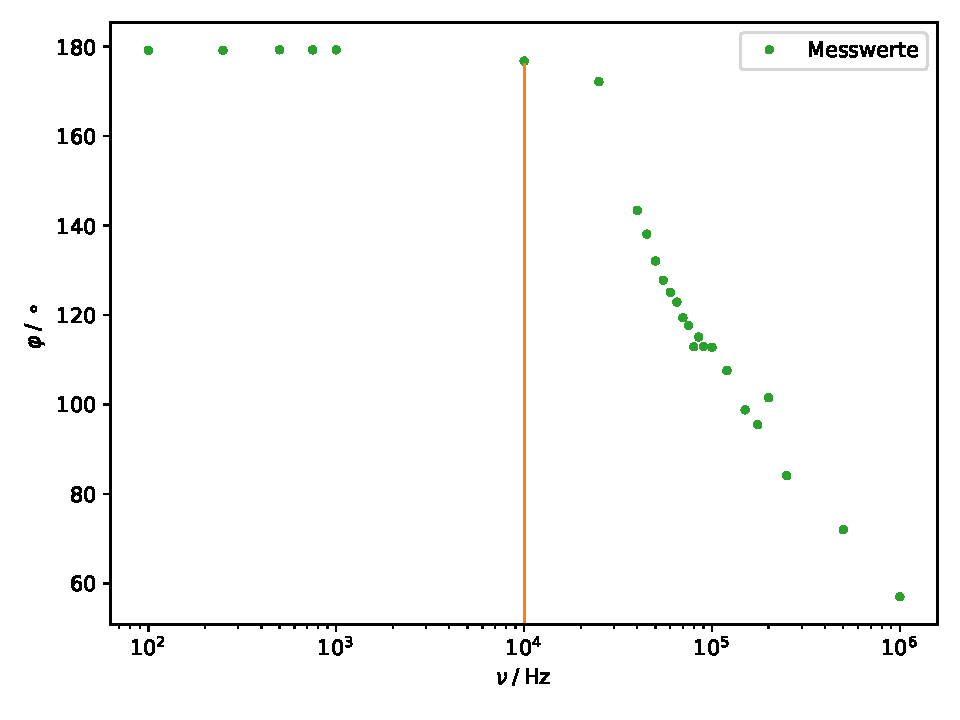
\includegraphics[width=0.65\textwidth]{Linearverstaerker_Anneke/phase.pdf}
  \caption{Phasenverschiebung zwischen der Ausgangs- und der Eingangsspannung $\varphi$ in Abhängigkeit der eingestellten Frequenz $\nu$. Es zeigt sich eine anfängliche Verschiebung um $\SI{180}{^\circ}$, die nach etwa $\SI{10}{kHz}$ abnimmt. Diese Grenze ist durch eine orangefarbene Linie gekennzeichnet.}
  \label{phase}
\end{figure}


% Die Untersuchung der verschiedenen Linearverstärker beginnt mit der Bestimmung der Grenzfrequenz $v'_g$. Hierzu wird die Ausgangsspannung gegen die Frequenz aufgetragen und danach die Anhängigkeit der Verstärkung von der Frequenz untersucht. Die Grenzfrequenz ist dann diejenige, bei welcher die Verstärkung $V'$ auf $\frac{V'}{\sqrt{2}}$ abgefallen ist.
% Die Widerstandswerte für die Linearverstärker sind in Tabelle \ref{Tab_2} zu finden. Der Ausgangsspannungsverlauf des ersten Verstärkers ist in Abb.\ref{plot1} dargestellt.
% \begin{figure}[h]
%   \centering
%   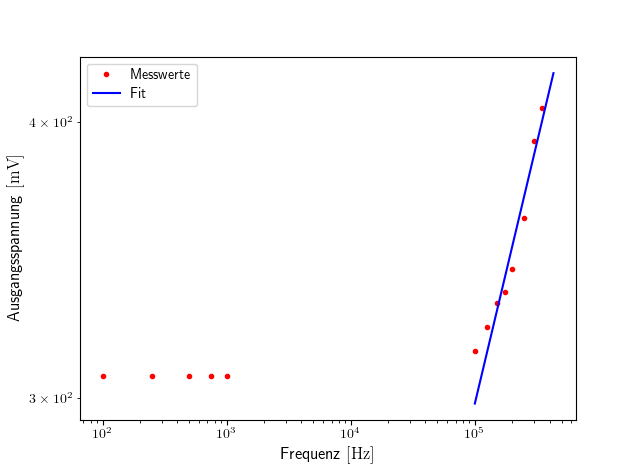
\includegraphics[width=1\textwidth]{bilder/Figure_1.png}
%   \caption{Frequenzverlauf der Ausgangsspannung mit Fit an der steigenden Seite.}
%   \label{Aufbau}
% \end{figure}
% Hierbei wird neben dem Darstellen der Messwerte noch ein Fit der Form
% \begin{equation}
% f(x)=mx^b
% \end{equation}
% durchgeführt um die Steigung der Gerade im doppeltlogarithmischen Plot zu bestimmen. Die Ergebnisse der Fits für die unterschiedlichen Linearverstärker sind in Tabelle \ref{Tab_1} eingetragen.
%
% \begin{figure}[h]
%   \centering
%   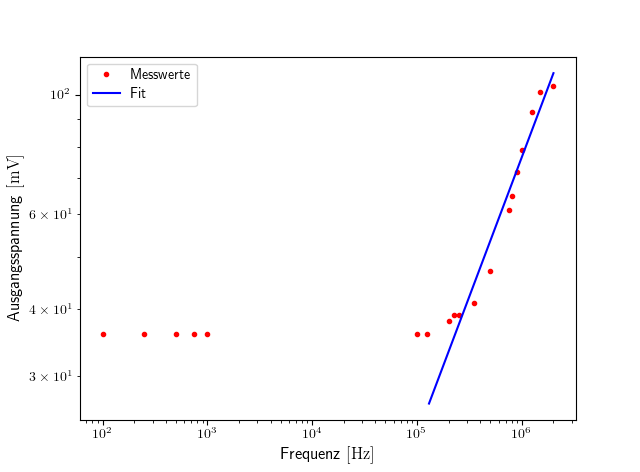
\includegraphics[width=1\textwidth]{bilder/Figure_2.png}
%   \caption{Frequenzverlauf der Ausgangsspannung des zweiten Linearverstärkers mit Fit an der steigenden Seite.}
%   \label{Aufbau}
% \end{figure}
% \begin{figure}[h]
%   \centering
%   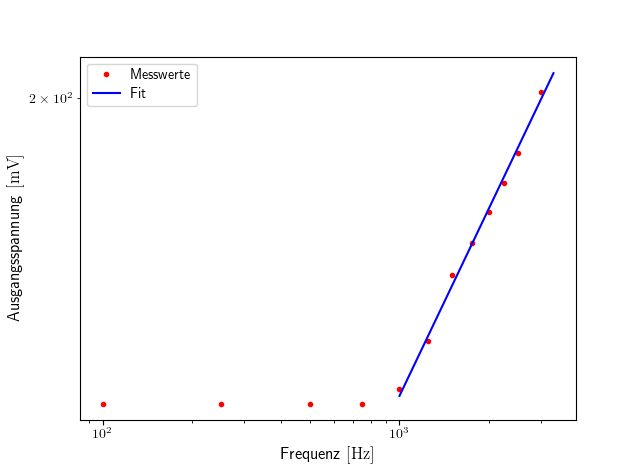
\includegraphics[width=1\textwidth]{bilder/Figure_3.png}
%   \caption{Darstellung des Frequenzverlaufs der Ausgangsspannung am dritten Linearverstärker mit Fit an der steigenden Seite.}
%   \label{Aufbau}
% \end{figure}
% \begin{figure}[h]
%   \centering
%   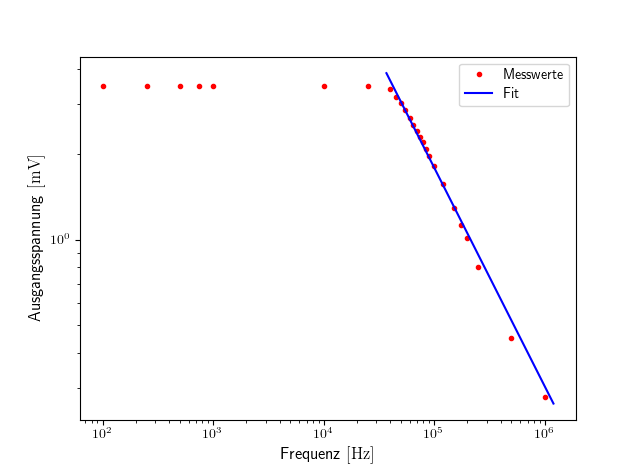
\includegraphics[width=1\textwidth]{bilder/Figure_4.png}
%   \caption{Frequenzabhängigkeit der Ausgangsspannung des vierten Linearverstärkers mit Fit an der fallenden Seite.}
%   \label{Aufbau}
% \end{figure}
% Es lässt sich nun die Grenzfrequenz für die einzelnen Linearverstärker bestimmen indem die Fitfunktion invertiert wird und der Frequenzwert für $U_A=\frac{U'_\text{const}}{\sqrt{2}}$, wobei $U'_\text{const}$ die Spannung am konstanten Teil der Kurve ist, berechnet wird:
% \begin{equation}
%   \nu_g=\left(\frac{U'_\text{const}}{\sqrt{2}m}\right)^{\frac{1}{b}}
% \end{equation}
% Es ergibt sich für die verschiedenen Linearverstärker
% \begin{table}[H]
% \centering
% \begin{tabular}{c|cc}
% &$m\,[\frac{\si{\mV}}{\si{\kHz}}]$&$b$\\
% \hline
% Verstärker 1 & $24\pm 9$ & $0{,}218\pm 0{,}031$\\
% Verstärker 2 & $0{,}61\pm0{,}3$ & $0{,}52\pm0{,}04$   \\
% Verstärker 3 & $27{,}4\pm2{,}0$ & $0{,}248\pm0{,}009$   \\
% Verstärker 4 & $(1{,}26\pm0{,}24)\cdot10^4$ & $-0{,}769\pm0{,}017$   \\
% \end{tabular}
% \label{Tab_3}
% \end{table}
%%%%%%%%%%%%%%%%%%%%%%%%%%%%%%%%%%%%%%%%%%%%%%%%%%
\subsection{Untersuchung des Umkehr-Integrators und Differentiators}
Es wird untersucht in welchem Bereich die theoretischen Zusammenhänge zwischen Ausgangsspannung und Frequenz erfüllt sind. Hierzu wird erneut die Ausgangsspannung für beide Aufbauten doppeltlogarithmisch gegen die Frequenz aufgetragen und die Steigung der auftretenden Gerade durch einen Fit ermittelt. Die Messwerte sowie die Ausgleichskurven sind in den Abb.\ref{integrator} und Abb.\ref{differentiator} dargestellt. Für beide Schaltungen wurde ein Kondensator mit einer Kapazität von $F=0{,}015\,\si{\micro\farad}$ und ein Widerstand mit $R=10\,\si{\kilo\ohm}$ genutzt. Für die Fitfunktion der Form:
\begin{equation}
\log(U_A)=m\cdot\log(\nu)+b\,,
\end{equation}
ergeben sich die Parameter:
\begin{align}
\text{Umkehr-Differentiator:}\nonumber\\
m&=\left(-0{,}81\pm0{,}02\right)\nonumber\\
b&=\left(5{,}18\pm0{,}06\right)\nonumber\\
\text{Umkehr-Integrator:}\nonumber\\
m&=\left(1{,}01\pm0{,}03\right)\nonumber\\
b&=\left(-0{,}6\pm0{,}2\right)\nonumber\\
\end{align}
\begin{figure}[h]
  \centering
  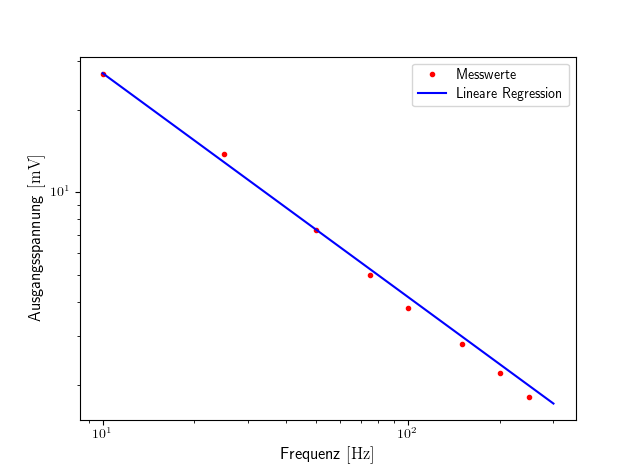
\includegraphics[width=1\textwidth]{bilder/innegrator.png}
  \caption{Die aufgenommenen Messwerte des Umkehr-Integrators mit linearer Regression}
\end{figure}
\begin{figure}[h]
  \centering
  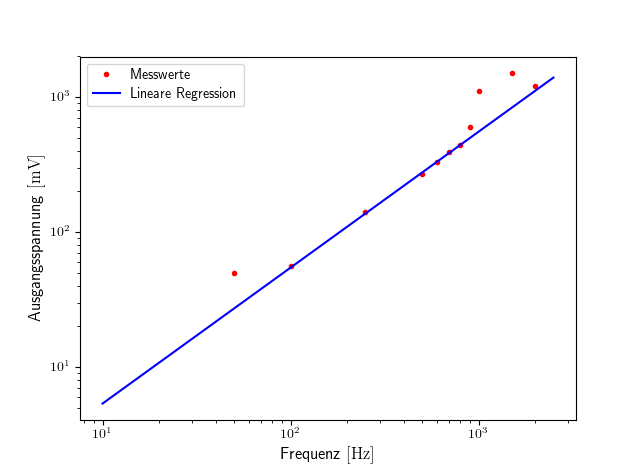
\includegraphics[width=1\textwidth]{bilder/diffe.png}
  \caption{Die aufgenommenen Messwerte des Umkehr-Differentiators mit linearer Regression}
\end{figure}
Für den Umkehr-Differentiator ist festzustellen, dass der erwartete Zusammenhang zwischen Ausgangsspannung und Frequenz nur zwischen ca. $100\,\si{\Hz}\.-\.800\,\si{\Hz}$ vorliegt. Beim Umkehr-Integrator hingegen findet sich kein Bereich in welchem der theoretische Verlauf nicht erfüllt wird. Die integrierenden und differentierenden Eigenschaften der Schaltungen sind in den folgenden Oszilloskopbildern gut zu erkennen, hierbei ist das Eingangssignal stets gelb un das Signal der Schaltung grün.
\begin{figure}[H]
  \centering
  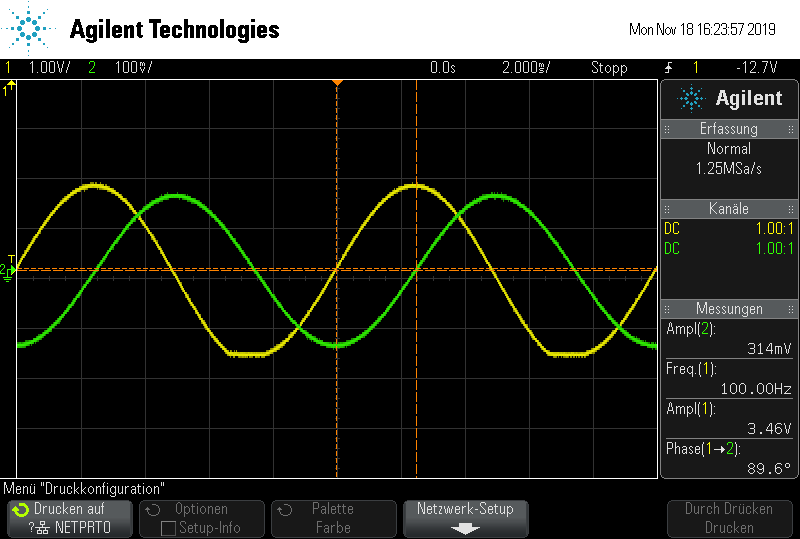
\includegraphics[width=1\textwidth]{bilder/integrator1.png}
  \caption{Integrierte Sinusspannung}
\end{figure}
\begin{figure}[H]
  \centering
  \includegraphics[width=1\textwidth]{bilder/integrator2.png}
  \caption{Integrierte Dreiecksspannung}
\end{figure}
\begin{figure}[H]
  \centering
  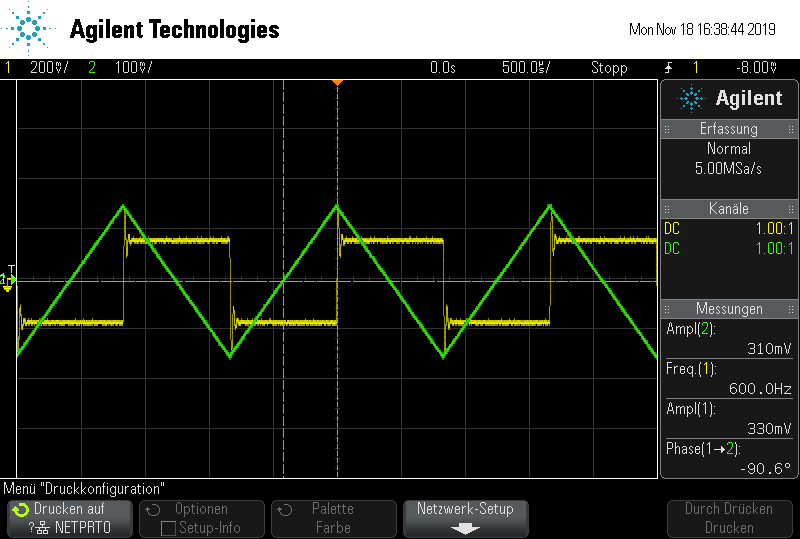
\includegraphics[width=1\textwidth]{bilder/integrator3.png}
  \caption{Integrierte Rechtecksspannung}
\end{figure}
\begin{figure}[H]
  \centering
  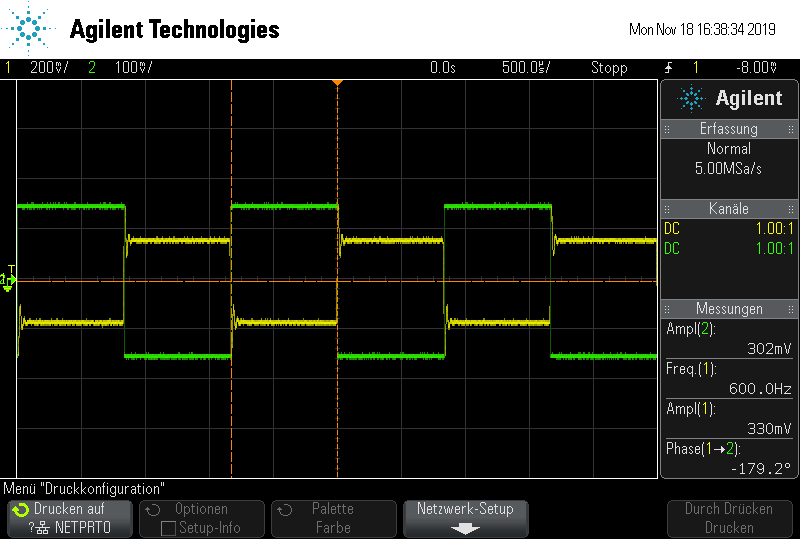
\includegraphics[width=1\textwidth]{bilder/diff1.png}
  \caption{Differentierte Rechtecksspannung}
\end{figure}
\begin{figure}[H]
  \centering
  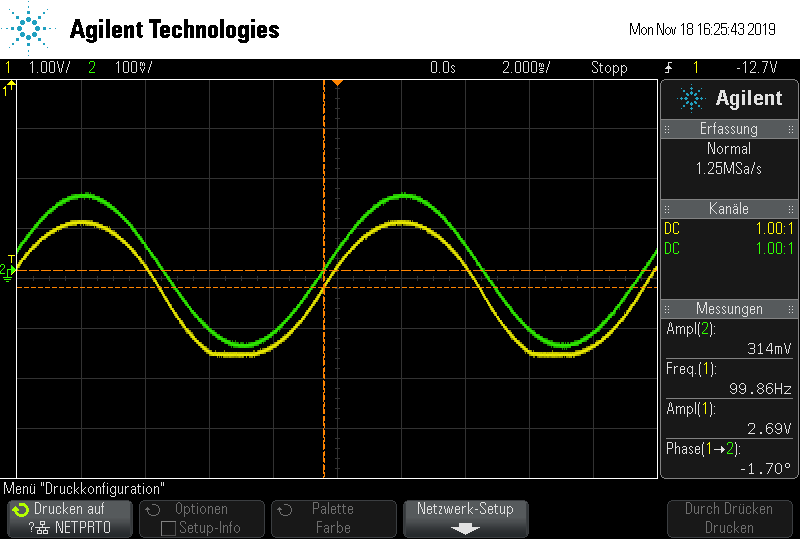
\includegraphics[width=1\textwidth]{bilder/diff2.png}
  \caption{Differentierte Sinusspannung?}%Vllt auch rausnehmen
\end{figure}
\subsection{Der Schmitt-Trigger}
Die technischen Daten des Aufbaus des Schmitt-Triggers sind:
\begin{table}[H]
\centering
\begin{tabular}{ccc}
$U_{B,+}=12{,}75 \,\si{\V}$ \\
$U_{B,-}=-13{,}8\,\si{V}$ \\
$R_1=10\,\si{\kilo\ohm}$ \\
$R_p=33\,\si{\kilo\ohm}$ \\
\end{tabular}
\end{table}
Mit (15) ergibt sich dann ein theoretischer Umschlagpunkt von
\begin{equation}
U_{+,\text{theo}}=3{,}86\,\si{\V}
\end{equation}
Der gemessene Schwellwert liegt bei
\begin{equation}
U_{+}=4{,}15\,\si{\V}
\end{equation}
Es liegt somit eine Abweichung von ca. $7\%$ vor.
